\section{Preamble}%
\label{sec:preamble_compound_types}

Before presenting the specifications of the different compound types, let's
define some useful language elements.


\begin{itemize}
\item \textit{Data borrowing} -- A data borrowing value is a value that points
  to data that is not automatically copied when the value is copied. The
  simplest example of data borrowing is the use of a pointer type, where the
  value of the pointer provides information about a memory address containing
  data. The data that the pointer points to is not copied when the pointer is
  copied. An illustration of this is given in figure~\ref{fig:data_borrowing}.
  In this example, both variables \texttt{x} and \texttt{y} borrow the data
  located on the heap at address \texttt{0xfa45b987}. Copying the value of the
  variable \texttt{y} to another variable does not make a copy of the borrowed
  value (which is on the heap), but only copies the value directly inside
  \texttt{y}, which in this case is on the stack. The borrowed data can be on
  the stack or on the heap, and the same can be said for the borrowing data.
  Such memory is called "borrowed" because it can live longer than the value
  pointing to it, and the pointer only temporarily borrows its value for reading
  or writing.

  In the case of borrowing data, mutability is crucial because multiple variables
  refer to the same segment of memory. This can lead to unpredictable side
  effects. Memory mutability is used to manage such behaviour and to ensure that
  only a few variables have mutable access to values. Most importantly, it is a
  safeguard against the accidental creation of mutable memory references.


\end{itemize}
\begin{figure}[H]
  \centering
  \begin{adjustbox}{max size=\linewidth}
    \begin{tikzpicture}
      % ================ Axis ========================
      \draw (0, 0) -- coordinate (LEFT) (0, 0);
      \draw[-Stealth](0, 10) -- coordinate (YAx) (0, 1.5);
      \draw[-Stealth](7.2, 10) -- coordinate (YAx) (7.2, 1.5);
      \draw[Box] (3.5, 10.7) -- (3.5, 10.7) node[anchor=center]{\textbf{STACK}};

      \filldraw (0, 6.5) circle (1pt) node[align=center, left] {+0};
      \filldraw (0, 5.5) circle (1pt) node[align=center, left] {+8};
      \filldraw (0, 4.5) circle (1pt) node[align=center, left] {+16};
      \filldraw (0, 3.5) circle (1pt) node[align=center, left] {+24};
      \filldraw (0, 2.5) circle (1pt) node[align=center, left] {+32};

      %% % ================ Foo ========================
      \fill[black!10] (0.2, 10) rectangle (7, 8);
      \draw[Box] (3.5, 7.6) -- (3.5, 7.6) node[anchor=center]{\textbf{.}};
      \draw[Box] (3.5, 7.4) -- (3.5, 7.4) node[anchor=center]{\textbf{.}};
      \draw[Box] (3.5, 7.2) -- (3.5, 7.2) node[anchor=center]{\textbf{.}};

      \draw[line width=1pt] (0.18, 6.9) rectangle (7.02, 2.48);
      \fill[olive!10] (0.2, 6.5) rectangle (7, 2.5);
      \draw[Box] (3.5, 6.7) -- (3.5, 6.7) node[anchor=center]{\emph{foo}};

      \draw[Box] (0.5, 5.5) -- (0.5, 5.5) node[anchor=center]{\textbf{\textit{x}}};
      \draw[line width=0.005pt] (0.3, 6.4) rectangle (6.8, 4.6);
      \draw[line width=0.005pt] (0.7, 5.5) rectangle (6.8, 5.5);

      \draw[Box] (3.5, 6) -- (3.5, 6) node[anchor=center]{\emph{len~=}~$3$};
      \draw[Box] (3.5, 5) -- (3.5, 5) node[anchor=center]{\emph{ptr~=}~0xfa45b987};

      \draw[Box] (0.5, 3.5) -- (0.5, 3.5) node[anchor=center]{\textbf{\textit{y}}};
      \draw[line width=0.005pt] (0.3, 4.4) rectangle (6.8, 2.6);
      \draw[line width=0.005pt] (0.7, 3.5) rectangle (6.8, 3.5);

      \draw[Box] (3.5, 4) -- (3.5, 4) node[anchor=center]{\emph{len~=}~$3$};
      \draw[Box] (3.5, 3) -- (3.5, 3) node[anchor=center]{\emph{ptr~=}~0xfa45b987};


      %% % ================ Heap ========================

      \draw[-Stealth](10, 10) -- coordinate (YAx) (10, 1.5);
      \draw[-Stealth](17.2, 10) -- coordinate (YAx) (17.2, 1.5);
      \filldraw (17.2, 7.5) circle (1pt) node[align=center, right] {0xfa45b987};

      % ================ Data ========================
      \draw[Box] (13.5, 10.7) -- (13.5, 10.7) node[anchor=center]{\textbf{HEAP}};
      \fill[black!10] (10.2, 10) rectangle (17, 8);
      \fill[teal!20] (10.2, 7.9) rectangle (17, 5);
      \draw[line width=0.005pt] (10.4, 7) rectangle (16.8, 7);
      \draw[line width=0.005pt] (10.4, 6) rectangle (16.8, 6);

      \draw[Box] (13.5, 7.5)  (13.8, 7.5) node[anchor=center]{$1$};
      \draw[Box] (13.5, 6.5)  (13.8, 6.5) node[anchor=center]{$2$};
      \draw[Box] (13.5, 5.5)  (13.8, 5.5) node[anchor=center]{$3$};

      \draw[thick,-Stealth,shorten >=1pt] (7.3, 5) to [out=0,in=180] node[below left, yshift=3mm] {} (9.9, 7.5);

      \draw[thick,-Stealth,shorten >=1pt] (7.3, 3) to [out=0,in=180] node[below left, yshift=3mm] {} (9.9, 7.5);

    \end{tikzpicture}
  \end{adjustbox}
  \vspace{-30pt}%
  \caption{\label{fig:data_borrowing}Example of data borrowing}
\end{figure}
%
%% \vspace{2pt}%

\begin{itemize}
\item \textit{Data movement} -- Data movement is the process of copying a value
  from one segment of memory to another. This can be done by allocation, memory
  copy (or deep copy), function calls and other operations. Data movements are
  always explicit, which ensures that no unwanted copies are made that could
  potentially slow down the program.

\item \textit{lvalue} -- An lvalue refers to the left operand in a \textit{data
  movement} operation. In other words, it is an expression that refers to a
  segment of memory that is modified as a result of the \textit{data movement}.
  An lvalue can take various forms, including a simple variable, a function
  parameter, an index operation, and more.

\item \textit{rvalue} -- An rvalue is the right operand involved in a
  \textit{data movement} operation. A rvalue can be aliased (using the keyword
  \texttt{alias}), referenced (keyword \texttt{ref}), copied with
  (\texttt{copy}, \texttt{dcopy}), or it can be implicit. Implicit means that
  the \textit{data movement} does not borrow mutable data and can therefore be
  allowed implicitly. In the case of an implicit \textit{data movement} there is
  no copying of borrowed data and there is no new borrowing of mutable memory.

\end{itemize}

\section{Pointers}%
\label{sec:pointer_type}

Pointers are values storing an address of memory. Pointer types are described
using the \texttt{*} token followed by a type (e.g. \texttt{*i32} describing a
pointer to a \texttt{i32} value). In the beta version of Ymir (compiler written
in c++) the operator \texttt{\&} was used, it was changed as it was also used to
refer to object instances that are in a way pointers but have very different
behavior.

\subsection {Literals}

The keyword \texttt{null} is used to describe a pointer pointing to nowhere.
This is the only literal that can be used as a pointer value.

\subsection {Construction}

To construct a pointer, the unary operator \texttt{\&} can be used on a lvalue
(for example, a variable). This operator returns the address of the value
referenced by the operand, i.e. \texttt{\&a} returns the address of the segment
of memory referenced by the variable \texttt{a}. For the sake of simplicity, we
can say that we are retrieving the address of the variable \texttt{a}.

\begin{lstlisting}[style=coloredverbatim]
let a = 12;
let b : *i32 = &a;
\end{lstlisting}

\subsection {Mutability}

Because pointers borrow data from another value (value pointed by the pointer),
their mutability is important. A pointer has two level of mutability:
\begin{enumerate}
\item \texttt{mut *T}, In this case, the pointer can be changed, but the value
  inside the pointer cannot be changed.
\item \texttt{mut *(mut T)}, In this case, both the value to which the pointer
  is pointing and the pointer itself can be changed.
\end{enumerate}

A mutable pointer (\textit{level 1}) means that if the pointer is contained
inside another compound type or variable, then the value it points to can be
changed. Checking for mutability is done at compile time when borrowing a value
to construct a pointer value.

\begin{lstlisting}[style=coloredverbatim]
let dmut a : *i32 = null;

let b = 12;
a = &b; // not allowed 'b' is not mutable
*a = 24; // but it would be modified by this operation


let mut c = 11;
a = &c; // allowed c is mutable
*a = 24; // modify the value of c is allowed
\end{lstlisting}

The keyword \texttt{alias} must be used on the right operand when data borrowing
is transferred to the left operand. In practice, this means that if the
mutability of the left operand is second level (i.e. \texttt{mut *(mut T)}), the
keyword \texttt{alias} must be used, and the right operand must also be second
level mutable. The keyword can be omitted if the aliasing is obvious (i.e. by
function return, or construction such as the unary operator \texttt{\&}).

\subsection {Properties}

Pointer type properties can be accessed using the \texttt{::} operator on a type
expression. The properties are as follows: following:

% \vspace{-20pt}%
\begin{center}\begin{adjustbox}{max width=\linewidth}
  \begin{tabular}{|l|ll|}
    \hline
    Name & Meaning & Type\\
    \hline
    \hline
    \texttt{init} & The initial value \texttt{null} & \texttt{typeof(x)}\\
    \hline
    \texttt{typeid} & A string encoding the name of the type & \texttt{[c8]} \\
    \hline
  \end{tabular}
\end{adjustbox}\end{center}

\subsection {Casting}

A pointer type can be cast to any pointer type using the cast operator
\texttt{cast!T(V)}. A pointer is a really low-level type with few guarantees,
but some operations rely on this possibility to perform generic operations
(common trait \texttt{Packable} for example). The mutability of the result is
the same as the mutability of the operand. This is the only allowed cast on
pointer types.

\subsection {Unary operators}

The unary operator \texttt{*} is used on a pointer value to dereference it and
access the value pointed to by the pointer. This operation is unsafe and may
cause the program to crash. If the operation does not crash, it does not
necessarily mean that the pointer was created correctly. This operation is
unsafe and can only be used in a \texttt{unsafe} context.

\begin{lstlisting}[style=coloredverbatim]
let i = 10;
let x = &i;

unsafe {
  let j = *x;
}
\end{lstlisting}

\subsection {Binary operators}

Binary operators are divided into 3 groups:
\begin{itemize}
\item Arithmetic: Pointer arithmetic is allowed with a \texttt{usize} as the
  right operand. Unlike the C language, the arithmetic does not depend on the
  size of the data pointed to by the pointer. The operation adds a number of
  bytes to the address, which means that the addition operation with a left
  operand whose value is \texttt{0xabc0} and a right operand \texttt{8us} will
  always have the value \texttt{0xabc8}, regardless of the type of content
  pointed to by the pointer. The behaviour is not the same with the index
  operator. The type of the result of the operation is always the same as the
  type of the left operand.

  %
  %\vspace{-14pt}%
  \begin{center}\begin{adjustbox}{max width=1\linewidth}
    \begin{tabular}{|c|lll|}
      \hline
      Operator & Operation & Commutative & Example \\
      \hline
      \hline
      \texttt{+} & Addition & Yes & \texttt{\&a + 2us} \\
      \texttt{-} & Substraction & No & \texttt{\&a - 2us} \\
      \hline
    \end{tabular}
  \end{adjustbox}\end{center}

\item Logical: Comparison operators always return a value of type \texttt{bool}
  and can only be used if the two operands are of the same pointer type (e.g.
  \texttt{*i32} with \texttt{*i32}).

  %\vspace{-15pt}%
  \begin{center}\begin{adjustbox}{max width=1\linewidth}
    \begin{tabular}{|c|lll|}
      \hline
      Operator & Operation & Commutative & Example \\
      \hline
      \hline
      \texttt{is} & Equality test & Yes & \texttt{\&a is \&a == true}\\
      \texttt{!is} & Equality test & Yes & \texttt{\&a !is \&a == false}\\
      \texttt{<} & Lower than & No & \texttt{\&a < \&a + 1us == false}\\
      \texttt{>} & Greater than & No & \texttt{\&a > \&a - 1us == false}\\
      \hline
    \end{tabular}
  \end{adjustbox}\end{center}

\item Affectation: The affectation operators are usable when the two operands
  are of exactly the same pointer type. The mutability level of the left operand
  must be less than or equal to the mutability level of the right operand.
  Affection operators can be mixed with arithmetic operators (e.g. \texttt{+=},
  \texttt{-=}). In this case the operation is rewritten as \texttt{x = x + y}
  and \texttt{y} must be a value of type \texttt{usize}.

  \begin{lstlisting}[style=coloredverbatim]
let mut a = 11;
let dmut b = &a;

let mut c = &a;
b = c; // not allowed it will discard the const property
c = b; // No problem the mutability level of c is lower than the one of b

c += 1us;

let dmut d = &a;
b = alias d; // alias is needed, data is borrowed
  \end{lstlisting}

\end{itemize}

\subsection {Index operator}

The index operator can be used on a pointer left operand with an int value as
the index right operand. The result of the operation is the dereferencing of the
pointer value by the offset of the value used as index. Unlike pointer
arithmetic using the \texttt{+} and \texttt{-} operators, the index operator
takes into account the size of the data pointed to by the pointer, i.e. the
index operation \texttt{(\&a)[7]} is strictly transformed into \texttt{*(\&a +
  (7us * sizeof (\_\_pragma!inner (typeof(\&a), 0)))}. This operation is unsafe because it
dereferences a raw pointer.

\smallskip

\begin{lstlisting}[style=coloredverbatim]
let mut a = 12;
let dmut b = &a;

unsafe {
  b [0] = 89;
}
assert (a == 89);
\end{lstlisting}

\smallskip

The mutability of the result value depends on the mutability level of the
pointer operand. If the mutability level of the pointer operand is 2, then the
result can be used as lvalue.

\section {Tuples}


Tuples are anonymous structures that store a set of data of different types.
They are described as a list of types enclosed in parentheses (e.g.
\texttt{(i32, f32, c8)}). A tuple may have only one inner type, in which case
the token \texttt{,} is added after the definition of the inner type (e.g.
\texttt{(i32,)}).

\subsection {Literals}

Tuple literals are described as a list of values enclosed in parentheses, for
example \texttt{(1, 'r', false)} is a tuple literal whose type is \texttt{(i32,
  c32, bool)}. Tuples containing only one value must have the token \texttt{,}
after the declaration of the value to distinguish them from priority operations
enclosed in parentheses.

\begin{lstlisting}[style=coloredverbatim]
let a = (1, 'r', false);
let b : (i32,) = (23,); // tuple value
let c : i32 = (23); // int value
\end{lstlisting}

\noindent Tuple inner values are constructed in the order in which they are
written. In the following example, the function \texttt{foo} is called before
the function \texttt{bar}.

\begin{lstlisting}[style=coloredverbatim]
fn foo ()-> i32 {
  println ("In foo.");
  12
}

fn bar ()-> f32 {
  println ("In bar.");
  34.0f
}

let a = (foo (), bar ());
\end{lstlisting}

\subsection {Mutability and memory alignment}%
\label{sec:tuple_mutability}

The mutability of tuple values cannot be described as a level of mutability, as
might be the case for other compound types. In the case of tuples, mutability is
defined as a tree, where each node of the tree depends on the mutability of its
parent. For example, the mutability of the following tuple type \texttt{mut (mut
  i32, f32, dmut *c8)} is shown in the figure~\ref{fig:tuple_mutability}.

\begin{figure}[H]
  \centering
  \scalebox{1.3}{
    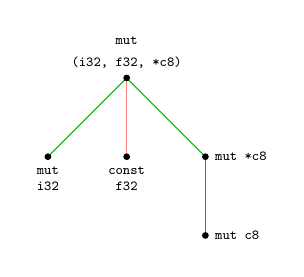
\begin{tikzpicture}

      \draw[-, black!30!green] (0,0) -- (-1,-1);
      \draw[-, red!50] (0,0) -- (0,-1);
      \draw[-, black!30!green] (0,0) -- (1,-1);
      \draw[-, black!30!green] (1,-1) -- (1,-2);

      \filldraw (0, 0.3) node[align=center, above] {\texttt{\tiny{mut}}};
      \filldraw (0, 0) circle (1pt) node[align=center, above] {\texttt{\tiny{(i32, f32, *c8)}}};
      \filldraw (-1,-1) circle (1pt) node[align=center, below]{\texttt{\tiny{mut}}};
      \filldraw (-1,-1.2) node[align=center, below]{\texttt{\tiny{i32}}};
      \filldraw (0,-1) circle (1pt) node[align=center, below]{\texttt{\tiny{const}}};
      \filldraw (0,-1.2) node[align=center, below]{\texttt{\tiny{f32}}};
      \filldraw (1,-1) circle (1pt) node[align=center, right]{\texttt{\tiny{mut *c8}}};
      \filldraw (1,-2) circle (1pt) node[align=center, right]{\texttt{\tiny{mut c8}}};


    \end{tikzpicture}
  }
  \caption{\label{fig:tuple_mutability} Example of tuple mutability}
\end{figure}


The mutability level of inner types is only important when they are borrowing
data. In the previous example shown in figure~\ref{fig:tuple_mutability}, only
the mutability of the inner type \texttt{*c8} is important during data movement.
In other words, a value of type \texttt{mut (i32, f32, dmut *c8)} can be passed
to it without any problem. As with any borrowing type, the keyword
\texttt{alias} must be used when borrowing data.

\begin{lstlisting}[style=coloredverbatim]
let mut x = 't'c8;
let mut a : mut (mut i32, f32, dmut *c8) = (1, 12.0f, &x);
let mut b : mut (i32, f32, dmut *c8) = (1, 7.0f, null);

a = alias b; // no problem
b = alias a; // no problem either

let c : (i32, f32, *c8) = (1, 7.0f, &x);
a = alias c; // not allowed, it would dicard constant property of the third field
\end{lstlisting}

Tuple types with mutable values that don't borrow data are considered
non-borrowing types, and therefore don't need \texttt{alias} during data
movement. In practice, all the data of such a tuple is copied during data
movement.

The alignment of tuples follows the same rules as the alignment of structures
(see chapter~\ref{chap:structures}), basically they are just anonymous
structures.

\subsection {Properties}

Pointer type properties can be accessed by using the \texttt{::} operator on a
type expression. The properties are as follows:
\smallskip

\begin{center}
  \begin{adjustbox}{max width=\linewidth}
    \begin{tabular}{|l|ll|}
      \hline
      Name & Meaning & Type\\
      \hline
      \hline
      \texttt{init} & The inital value of the tuple & \texttt{usize} \\
      & where every inner field are set to \texttt{T::init} & \\
      \Xhline{0.001pt}
      \texttt{arity} & The number of inner elements of the tuple type & \texttt{usize}\\
      \hline
      \texttt{init} & A string encoding the name of the type & \texttt{[c8]} \\
      \hline
    \end{tabular}
  \end{adjustbox}
\end{center}

\smallskip

Inner types are not accessible using the \texttt{::} operator, but are
accessible using \texttt{\_\_pragma}. Pragmas are presented in the
section~\ref{sec:pragmas}.

\subsection {Binary operators}

Binary operators are divided into 3 groups:
\begin{itemize}
\item Access: The operator \texttt{.} is used to access a given field of the
  tuple. The right operand must be of type int and must be within the range of
  \texttt{0} and the arity of the tuple to be accessed. The result of the
  operation takes the type of the field at the index described by the right
  operand, and so does the value. The first field index is \texttt{0}.

  \begin{lstlisting}[style=coloredverbatim, linewidth=0.95\linewidth]
let mut a : (mut i32, f32) = (8, 8.f);

a._0 = 7; // allowed first field is mutable
a._1 = 1.f; // not allowed, second field is not mutable

let c = a.(12 - 11); // accessing the field at index 1
  \end{lstlisting}

\item Comparison: The comparison operators \texttt{==} and \texttt{!=} are
  defined on tuples when each of the inner types are comparable. It compares all
  fields of two tuples and checks whether all inner values are equal for
  \texttt{==} or at least one inner value is different between the two operands
  for the operator \texttt{!=}.

  There is no relation of order between the tuples, even if they are of the same
  type, since in general such a comparison would be meaningless.

\item Affectation: The affectation operator creates a \textit{data movement}
  from the right operand to the left operand. Mutability must be respected when
  data is borrowed. Data mutability on tuples has already been introduced in
  section~\ref{sec:tuple_mutability}.

\end{itemize}

\subsection {Dollar operator}

The dollar operator can be used within an access binary operation in the right
operand expression. The dollar value takes the value of the arity of the tuple,
and its type is \texttt{usize}. Its value is known at compile time.

\begin{lstlisting}[style=coloredverbatim]
let a = (1, 9.0f, 'r');

let b = a.($ - 1us); // access the last value, i.e. 'r'
\end{lstlisting}

\subsection {Tuple expansion}

Tuples have a special operator called \texttt{expand} that turns them into a
list of parameters. Expanding a tuple is useful to create other tuples, or to
pass the data of the tuple as function parameters.

\begin{lstlisting}[style=coloredverbatim]
fn foo (a : i32, b : f32) {}

let a = (1, 5.f);

 // transform a into a list of values
let b : (i32, f32, c32) = (expand a, 't');

foo (expand a); // transform a into a list of parameters
\end{lstlisting}

Such an operation is done at compile time and is simply a rewrite that is less
verbose. In fact, in the previous example, the line \texttt{foo (expand a)} is
rewritten as \texttt{foo (a.0, a.1)}. The mutability level of the expanded
values is always \texttt{1}, which means that tuple expansion can never borrow
mutable data. Tuple expansions are useful in variadic template functions to
write generic operations on a list of variadic parameters.

\subsection {Tuple deconstruction}

Tuple can be used to declare several variables at once, using the same
\texttt{let} declaration. We call this declaration a tuple deconstruction
because it splits the values of the tuple into a list of variables.

\begin{lstlisting}[style=coloredverbatim]
  // a is mutable, but not b nor c
let (mut a, b, c) = (1, 't', 12.f);

assert (a == 1 && b == 't' && c == 12.f);
\end{lstlisting}

A variadic variable can be used as the last variable declaration in such a
deconstruction with the token \texttt{...}. In this case, it's type is always a
tuple that takes all the values in the tuple that are left and not associated
with other variables.

\begin{lstlisting}[style=coloredverbatim]
let (a, b...) = (1, 2, 3);

assert (a == 1);
assert (b == (2, 3));

let (c, d...) = (1, 2);

assert (c == 1);
assert (d == (2,));
\end{lstlisting}

The mutability level of variables declared using tuple deconstruction can be
mutable by using the keywords \texttt{mut} or \texttt{dmut} on specific
variables of the tuple deconstruction (i.e. \texttt{let (dmut a, b) = alias
  t;}). In that case the right operand must match the mutability, and be aliased
explicitly.

\subsection {Tuple iteration}

Tuples are iterable types, so they can be used as the iterable value of a
\texttt{for} loop. In practice, because such an iteration would create iterator
variables of different types, the iteration is unrolled at compile time. The
tuple value is only constructed once before entering any loop body.

\begin{lstlisting}[style=coloredverbatim]
let a = (1, 't', 89.0f);
for i in a {
    println (i);
}

// would be rewritten into
println (a._0);
println (a._1);
println (a._2);
\end{lstlisting}

Two variables can be used as iterators, the first being the index of the
iteration and the second being the value within the tuple. If only one variable
is defined, only the value of the tuple fields is contained in the iterator.
Iterators are always immutable and never used as references, but this limitation
can easily be circumvented by using the index iterator to access the tuple.

\begin{lstlisting}[style=coloredverbatim]
let dmut a = (1, 2, 3);
for i, _ in a {
    a.(i) = 9;
}

assert (a == (9, 9, 9));
\end{lstlisting}

More information about \texttt{for} loops is presented in Section~\ref{sec:for_loops}.

\section {Ranges}%
\label{sec:range_type}

Range is a compound type consisting of four elements that describe a range of
values. The four elements are \texttt{fst} the first value of the range (e.g.
\texttt{0}), \texttt{scd} the last value of the range (e.g. \texttt{10}),
\texttt{step} the step of the range (e.g. \texttt{2}), and \texttt{contains} of
type bool, which indicates whether the last value \texttt{scd} is contained in
the range or not. There are only three types that can describe the inner
components of a range: integer, floating point and character. The type of the
range is defined by the inner type followed by the token \texttt{..} (e.g.
\texttt{i32..} describes a range of \texttt{i32} values). Range are useful for
iteration or for accessing a subset of values (for example, a subset of a
slice).

\subsection {Literals}

Range literals are described using the \texttt{..} token or the \texttt{...}
token. The \texttt{..} token is used to define a range whose final value is not
included in the range, and the \texttt{...} token defines a range whose final
value is included. If different tokens are used to describe the literal, the
type is the same, and the \texttt{..} token is always the only token used to
describe a range type.

\begin{lstlisting}[style=coloredverbatim]
let a : i32.. = 0 .. 2;
let b : i32.. = 0 ... 2;

assert (a.fst == b.fst);
assert (a.scd == b.scd);
assert (a.step == b.step);
assert (!a.contains && b.contains);
\end{lstlisting}

Range values can be decreasing, in which case the step is negative. Note that
for ranges of unsigned integers and character values, it is theoretically
impossible to have a negative value for the step. However, there is a bit of
cheating going on here, using the overflow limitation of types to create a value
that, when added to \texttt{fst}, equals \texttt{fst - abs (step)} (in practice,
this is exactly the same as adding a negative value at the binary level, but it
is not really the valid high level representation). For this reason it can be
considered that step is always a signed version of the type, even if the field
type is considered to be the same as the type of the inner values (\texttt{fst}
and \texttt{scd}), and thus one bit of its encoding is always used for the sign.

The \texttt{fst} value of the range literal is constructed before the
\texttt{scd} value. In the following example, the function \texttt{foo} is
called before the function \texttt{bar}.

\begin{lstlisting}[style=coloredverbatim]
fn foo ()-> i32 {
  println ("In foo.");
  12
}

fn bar ()-> i32 {
  println ("In bar.");
  1
}

let a = (foo ()) .. (bar ());
\end{lstlisting}

\subsection {Mutability and memory alignement}

As expected, range values do not share any data, and every field included in the
value is replicated during data movement. Therefore, there is no concern for
mutability, rendering the type not aliasable. A mutable range has the ability to
modify its internal fields, but even if the range type is a compound type, it
operates precisely like a scalar type since it can never contain any borrowed
data. In memory a range value has the same memory alignement as the structure
(cf. Chapter~\ref{chap:structures}) presented in the following source code where
\texttt{T} is the inner type of the range.

\begin{lstlisting}[style=coloredverbatim]
struct {T}
| fst : T
| scd : T
| step : T
| contains : bool
-> Range;
\end{lstlisting}

\subsection {Properties}

Range type properties can be accessed through the operator \texttt{::} applied
to a type expression. The following properties include:

\begin{center}\begin{adjustbox}{max width=\linewidth}
  \begin{tabular}{|l|ll|}
    \hline
    Name & Meaning & Type\\
    \hline
    \hline
    \texttt{init} & The initial value ranging from \texttt{T::init} & \texttt{typeof (x)}\\
    & to \texttt{T::init} with a step of \texttt{T::init} and & \\
    & with contains set to \texttt{false} where \texttt{T} is & \\
    & the inner type (e.g. \texttt{i32} for \texttt{i32..}). &\\
    \hline
    \texttt{typeid} & A string encoding the name of the type & \texttt{[c8]} \\
    \hline
  \end{tabular}
\end{adjustbox}\end{center}


\subsection {Binary operators}

Binary operators are divided into 4 groups:

\begin{itemize}
\item Access: The operator \texttt{.} is utilized to access the field of the
  range type. The right operand is the name of the field to access. The fields
  are listed in the table below.

  %\vspace{-20pt}%
  \begin{center}\begin{adjustbox}{max width=\linewidth}
    \begin{threeparttable}
      \begin{tabular}{|l|ll|}
        \hline
        Name & Value & Type\\
        \hline
        \hline
        \texttt {fst} & The first value of the range & \textit{T}$^{1^{\phantom{j}}}$ \\
        \texttt {scd} & The second value of the range & \textit{T}$^{1^{\phantom{j}}}$ \\
        \texttt {step} & The step of the range & \textit{S}$^{2^{\phantom{j}}}$ \\
        \texttt {contains} & The field describing wether or  & \texttt{bool} \\
        & not the scd value is contained in the range &\\
        \hline
      \end{tabular}
      \begin{tablenotes}
      \item[1.] \texttt{\_\_pragma!inner (typeof (x), 0)}
      \item[2]\small \textit{Signed version of inner type for integer type
        ranges, an integer type for character type ranges, and
        \texttt{\_\_pragma!inner (typeof(x), 0)} for float type ranges.}
      \end{tablenotes}
    \end{threeparttable}
\end{adjustbox}\end{center}

Accessed fields are only mutable if the range is also mutable.

\item Contains: The \texttt{in} and \texttt{!in} operators verify the presence
  of a value in a range. The left operand must match the inner type of the right
  operand, and the right operand must be a range type.

\item Comparison: Ranges can be compared using the operators \texttt{==} and
  \texttt{!=}. This checks the equality or inequality of each field within the
  range. It is important that the left and right operands are of the same type.

\item Affectation: A range value can be an lvalue if and only if it is mutable.
  \begin{lstlisting}[style=coloredverbatim]
let mut a = 0 .. 7;

a = 7 .. 1;
  \end{lstlisting}

\end{itemize}

\subsection {Range iteration}

 Ranges are iterable types, so they can be used as the iterable value of a
 \texttt{for} loop. Only one immutable variable can be declared when iterating
 over a range value. This iterator variable takes the value of the \texttt{fst}
 field of the range and increments by the \texttt{step} field until it reaches
 the \texttt{scd} field. If the range is a containing range (i.e. the
 \texttt{contains} field is true), then the \texttt{scd} field is included in
 the iteration. Optimisations are performed if the inner values of the range are
 known at compile time.

\begin{lstlisting}[style=coloredverbatim]
for i in 0 .. 7 {
    print (i, ' '); // 0 1 2 3 4 5 6
}

for i in 0 ... 7 {
    print (i, ' '); // 0 1 2 3 4 5 6 7
}

for i in 7 .. 0 {
    print (i, ' '); // 7 6 5 4 3 2 1
}
\end{lstlisting}

 For more information on \texttt{for} loops, see the section~\ref{sec:for_loop}.

\section{Arrays}

 An array is a compound type containing a list of values of the same type stored
 in a contiguous memory segment and whose size is known at compile time. An
 array type is described using the following syntax \texttt{[T ; N]} where
 \texttt{T} is the inner type of the array and \texttt{N} is an integer value
 describing the number of elements contained in the array.

\subsection {Literals}

Array literals are a list of values enclosed in brackets \texttt{[} and
  \texttt{]}. An array literal of the size \texttt{0} does not contain any data
and consists only of the brackets. Array literals are indistinguishable from
slice literals (see section~\ref{sec:slices}), it is the type of the lvalue
operand that determines whether a slice or an array value is created. By
default, if the type of the lvalue is not defined, the operand type is always a
slice type.

\begin{lstlisting}[style=coloredverbatim]
fn foo (x : [i32 ; 4]) {
  // ...
}

let a = [1, 2, 3]; // slice [i32]
let b : [i32 ; 3] = [1, 2, 3]; // array [i32 ; 3]


foo ([1, 2, 3, 4]); // calling with an array [i32 ; 4]
\end{lstlisting}

Array literals can also be defined using the array construction syntax. The
syntax is similar to the type description of the array type, but uses a value
instead of a type \texttt{[V ; N]}. Each element of the array will take the
value \texttt{V}.

\begin{lstlisting}[style=coloredverbatim]
let a = [12 ; 2]; // an array of i32 of size 2, where every element is equal to 12

assert (a [0] == 12 && a [1] == 12);
\end{lstlisting}

Array inner values are constructed in the order in which they are written. In
the following example, the function \texttt{foo} is called before the function
\texttt{bar}.

\begin{lstlisting}[style=coloredverbatim]
fn foo ()-> i32 {
  println ("In foo.");
  1
}

fn bar ()-> i32 {
  println ("In bar.");
  2
}

let a : [i32 ; 2] = [foo (), bar ()];
\end{lstlisting}

When the syntax of the array allocation is used, the inner value is constructed
only once and is replicated at each index of the array. In the following
example, the function \texttt{foo} is called once and each index of the array
contains the value \texttt{12}.

\begin{lstlisting}[style=coloredverbatim]
fn foo ()-> i32 {
  println ("In foo.");
  12
}

let a = [foo () ; 4];
\end{lstlisting}

\subsection {Mutability and memory alignement}

Arrays don't borrow data themselves, because the data is actually the data of
the arrays themselves. This means that when data is moved, all the data
contained in an array is copied. As with tuples, the mutability level of an
array is therefore only important if the inner type of the array is a type that
borrows data. The memory representation of the following example is shown in
figure~\ref{fig:data_repr_array}.

\begin{lstlisting}[style=coloredverbatim]
let dmut a : [i32 ; 3] = [1, 2, 3];

let dmut b = a; // no need for alias
                // a and b don't refer to the same memory segment

let i = 89;
let c : [*i32 ; 1] = [&i];

let dmut d = c; // not allowed, discard const property of the inner type
\end{lstlisting}

\begin{figure}[H]
  \centering
  \scalebox{0.7}{
    \begin{tikzpicture}
      % ================ Axis ========================
      \draw (0, 0) -- coordinate (LEFT) (0, 0);
      \draw[->](0, 10) -- coordinate (YAx) (0, 0);
      \draw[->](7.2, 10) -- coordinate (YAx) (7.2, 0);
      \draw[Box] (3.5, 10.7) -- (3.5, 10.7) node[anchor=center]{\textbf{STACK}};

      \filldraw (0, 8) circle (1pt) node[align=center, left] {+0};
      \filldraw (0, 7.3) circle (1pt) node[align=center, left] {+4};
      \filldraw (0, 6.5) circle (1pt) node[align=center, left] {+8};
      \filldraw (0, 5.8) circle (1pt) node[align=center, left] {+12};
      \filldraw (0, 5.1) circle (1pt) node[align=center, left] {+16};
      \filldraw (0, 4.4) circle (1pt) node[align=center, left] {+20};
      \filldraw (0, 3.7) circle (1pt) node[align=center, left] {+24};
      \filldraw (0, 3) circle (1pt) node[align=center, left] {+28};
      \filldraw (0, 2.3) circle (1pt) node[align=center, left] {+32};
      \filldraw (0, 1.6) circle (1pt) node[align=center, left] {+36};
      \filldraw (0, 1) circle (1pt) node[align=center, left] {+40};

      %% % ================ Foo ========================
      \fill[black!10] (0.2, 10) rectangle (7, 9.5);
      \draw[Box] (3.5, 9.2) -- (3.5, 9.2) node[anchor=center]{\textbf{.}};
      \draw[Box] (3.5, 9) -- (3.5, 9) node[anchor=center]{\textbf{.}};
      \draw[Box] (3.5, 8.8) -- (3.5, 8.8) node[anchor=center]{\textbf{.}};

      \draw[line width=1pt] (0.18, 8.5) rectangle (7.02, 0.95);
      \fill[olive!10] (0.2, 8) rectangle (7, 0.95);
      \draw[Box] (3.5, 8.2) -- (3.5, 8.2) node[anchor=center]{\emph{foo}};

      \draw[Box] (0.5, 6.95) -- (0.5, 6.95) node[anchor=center]{\textbf{\textit{a}}};
      \draw[line width=0.005pt] (0.3, 7.95) rectangle (6.8, 5.95);

      \draw[Box] (3.5, 7.65) -- (3.5, 7.65) node[anchor=center]{$1$};
      \draw[Box] (3.5, 6.95) -- (3.5, 6.95) node[anchor=center]{$2$};
      \draw[Box] (3.5, 6.25) -- (3.5, 6.25) node[anchor=center]{$3$};

      \draw[Box] (0.5, 4.85) -- (0.5, 4.85) node[anchor=center]{\textbf{\textit{b}}};
      \draw[line width=0.005pt] (0.3, 5.75) rectangle (6.8, 3.85);

      \draw[Box] (3.5, 5.5) -- (3.5, 5.5) node[anchor=center]{$1$};
      \draw[Box] (3.5, 4.8) -- (3.5, 4.8) node[anchor=center]{$2$};
      \draw[Box] (3.5, 4.1) -- (3.5, 4.1) node[anchor=center]{$3$};

      \draw[Box] (0.5, 3.4) -- (0.5, 3.4) node[anchor=center]{\textbf{\textit{i}}};
      \draw[line width=0.005pt] (0.3, 3.65) rectangle (6.8, 3.15);
      \draw[Box] (3.5, 3.4) -- (3.5, 3.4) node[anchor=center]{$89$};

      \draw[Box] (3.5, 2.7) -- (3.5, 2.7) node[anchor=center]{-};

      \draw[Box] (0.5, 1.6) -- (0.5, 1.6) node[anchor=center]{\textbf{\textit{c}}};
      \draw[line width=0.005pt] (0.3, 2.35) rectangle (6.8, 1.05);
      \draw[Box] (3.5, 1.6) -- (3.5, 1.6) node[anchor=center]{\emph{ptr~=}~$foo+24$};

      \draw[-Stealth, thick, shorten >=0.2pt] (7.3, 1.6) to [out=-10,in=20, bend right=45] node[below left, yshift=1mm] {} (7.3, 3.4);

    \end{tikzpicture}
  }
  \caption{\label{fig:data_repr_array} Example of memory representation of array values}
\end{figure}


\subsection {Properties}

Array type properties can be accessed using the \texttt{::} operator on a type
expression. The properties are as follows:

%\vspace{-20pt}%
\begin{center}\begin{adjustbox}{max width=\linewidth}
  \begin{tabular}{|l|ll|}
    \hline
    Name & Meaning & Type\\
    \hline
    \hline
    \texttt{init} & The initial value, where all & \texttt{typeof(x)} \\
    & inner values are set to  & \\
    \Xhline{0.001pt}
    \texttt{size} & The static size of the array (is equal to \texttt{.len}) & \texttt{usize} \\
    \hline
    \texttt{typeid} & A string encoding the name of the type & \texttt{[c8]} \\
    \hline
  \end{tabular}
\end{adjustbox}\end{center}

\subsection {Binary operators}

Binary operators are divided into four groups:

\begin{itemize}
\item Access: The \texttt{.} operator is used to access fields that describe the
  array value. The right operand is the name of the field to be accessed. These
  fields are described in the table below.

  %\vspace{-20pt}%
\begin{center}\begin{adjustbox}{max width=\linewidth}
  \begin{tabular}{|l|ll|}
    \hline
    Name & Value & Type\\
    \hline
    \hline
    \texttt{len} & The size of the array & \texttt{usize} \\
    \texttt{ptr} & The pointer to the first element  & \texttt{*(\_\_pragma!inner (typeof (x), 0)} \\
    & of the array & \\
    \hline
  \end{tabular}
\end{adjustbox}\end{center}

The \texttt{len} field is known at compile time and can therefore be used in
a \texttt{cte} expression. The type of the \texttt{ptr} field has the same
level of mutability as the array type. Note that array does not really have
fields. The values are constructed from the array information, \texttt{ptr}
takes the address of the array as a value, and \texttt{len} is an integer
literal containing the length of the array in number of elements contained.

\item Concatenation: The concatenation operator \texttt{\~} is used to create an
  array or slice containing the values of two arrays or slices. The operator can
  be used if the left and right operands have the same internal type, regardless
  of their relative sizes. The mutability of the generated value is the
  strictest mutability between the two operands. For example, the type and
  mutability of \texttt{([*i32 ; 4]) \~\ (dmut [*i32 ; 2])} is \texttt{[*i32 ;
      6]} to avoid discarding the constant property of the values contained in
  the left operand. Notice that the type of the generated value is an array
  whose size is the sum of the left and right operand sizes.

  The operator can also be used when one of the operands is a slice. In this
  case, the return value of the operation will be a slice instead of an array,
  since its size cannot be known at compile time. This operation is actually
  performed more by the slice operand than by the array operands, and is
  discussed further in the section~\ref{sec:slices}.

  The operator \texttt{\~} was chosen to avoid confusion with \texttt{+}, which
  would behave differently depending on the operands.Concatenation is not really
  an arithmetic operation, as \texttt{+} would refer to an addition of all the
  inner values of two arrays, rather than their concatenation. Concatenation
  operator is obviously not commutative.

  \begin{lstlisting}[style=coloredverbatim]
let a : [i32 ; 3] = [1, 2, 3];
let b : [i32 ; 2] = [4, 5];

let c : [i32 ; 5] = a ~ b;

assert (c == [1, 2, 3, 4, 5]);
  \end{lstlisting}

\item Comparison: Binary comparison operators can be used with two arrays of the
  same inner type, or an array and a slice of the same inner type. The result of
  the operation is always of type \texttt{bool}. For the operators to work, the
  inner type of the array must also define the comparison operators. Lexical
  order is used, so the size of the arrays are only used if one of the two operands
  is a prefix of the other (e.g. \texttt{[1, 2]} is a prefix of \texttt{[1, 2,
      3]}, so \texttt{[1, 2, 3]} is considered greater than \texttt{[1, 2]}, but
  \texttt{[1, 3]} is greater than \texttt{[1, 2, 3]}).

  %\vspace{-20pt}%
  \begin{center}\begin{adjustbox}{max width=1.0\linewidth}
    \begin{tabular}{|c|lll|}
      \hline
      Operator & Operation & Comm. & Example\\
      \hline
      \hline
      \texttt{>}      & Greater than     & No          & \texttt{([1, 2] > [2, 3]) == false}    \\
      \texttt{<}      & Lower than       & No          & \texttt{([1, 2] < [2, 3]) == true}     \\
      \texttt{>=}     & Greater or equal & No          & \texttt{([1, 2, 3] >= [1, 2]) == true} \\
      \texttt{<=}     & Lower or equal   & No          & \texttt{([1, 2, 3] <= [2]) == true}    \\
      \texttt{==}     & Equal            & Yes         & \texttt{([1, 2] == [1, 2]) == true}    \\
      \texttt{!=}     & Not equal        & Yes         & \texttt{([1, 2] != [1, 2]) == false}   \\
      \hline
    \end{tabular}
  \end{adjustbox}\end{center}

\item Affectation: An array value can be an lvalue if and only if it is mutable.
  Information about inner type mutability has already been discussed in the
  section on mutability, and will therefore not be discussed further here. The
  size of the left and right operands must of course be strictly equal.

  \begin{lstlisting}[style=coloredverbatim]
let mut a : [i32 ; 2] = [1, 2];

a = [2, 3];
  \end{lstlisting}

\end{itemize}

\subsection {Index operator}

The index operator can be used on an array as the left operand, with an int
value or a range value as the right operand.

\begin{itemize}
\item With an int value; The element at the index described by the int value is
  returned. The mutability of the result value depends on the mutability of the
  inner type of the array. If the mutability level of the array type is at least
  \texttt{2}, the result value can be used as lvalue.

  \begin{lstlisting}[style=coloredverbatim]
let mut a : [mut i32 ; 3] = [1, 2, 3];
let mut b : [i32 ; 2] = [4, 5];

a [0] = 9; // ok, mutability level of 'a' is high enough

b [0] = 11; // not allowed, b inner values are not mutable
b = [9, 10]; // ok, b is mutable
  \end{lstlisting}

  If the value of the int operand is known at compile time, a size check is
  performed to ensure that the access does not overflow the array size, and that
  the value used is greater than or equal to zero. If the value is unknown at
  compile time, a condition is added and an array size check is performed at
  runtime. Panic is triggered if an overflow occurs.


\item With a range value; using a range value containing int values as the right
  operand, the program creates a slice containing only a subset of the array
  values. The mutability level of the created slice type is the same as the
  mutability of the array type. The \texttt{copy} operator must be used to create
  the slice value, as it allocates memory on the heap (see Slice
  limitation~\ref{sec:slice_lim}) and to prevent implicit memory allocations.

  \begin{lstlisting}[style=coloredverbatim]
let a = [i32 ; 4] = [1, 2, 3, 4];

let b : [i32] = copy a [0 .. 2];
  \end{lstlisting}

  If the inner values of the range are known at compile time, it is checked that
  there will be no array overflow. The range must be ascending, i.e. the first
  value of the range must be less than the second value. This is also checked at
  compile time if possible. If the values of the range are not known at compile
  time, then these checks are done at runtime. The contain field of the range
  has no effect on the array access, and the \texttt{scd} value is always
  considered not contained.

  If the range used to index the array is known at compile time, a new array
  value can be created. In that case the \texttt{copy} operator is no more
  mandatory, and the result of the operand is an array value.

  \begin{lstlisting}[style=coloredverbatim]
fn foo (a : [i32 ; 3]) {
  println (a);
}

let a = copy [1, 2, 3, 4];
foo (a [1 .. 4]);
  \end{lstlisting}

\end{itemize}

\subsection {Dollar operator}

The dollar operator can be used within an index operation in the right operand
expression. The dollar value takes the value of the size of the array and its
type is \texttt{usize}. Its value is known at compile time.

\begin{lstlisting}[style=coloredverbatim]
let a = [i32 ; 4] = [1, 2, 3, 4];

let b = copy a [0us .. $ - 1us]; // all the values except the last one

let c = a [$ - 2us]; // The second value to the last
\end{lstlisting}

\subsection {Array iteration}

Arrays are iterable types, so they can be used as iterable values of a
\texttt{for} loop. The \texttt{for} loop can use either one or two variables as
iterators. If a single variable is used, it automatically captures the value of
the array element at the current iteration index. Conversely, if two variables
are used, the first variable represents the iteration index, while the second
variable stores the value of the array element at that specific index.

\begin{lstlisting}[style=coloredverbatim]
let a : [i32 ; 4] = [1, 2, 3, 4];
for i, elem in a {
    assert (a [i] == elem);
}
\end{lstlisting}

If the inner values of an array are mutable, the element iterator can be used by
reference. The mutability of the iterator is the mutability of the inner type of
the array, or the mutability defined in the type declaration of the iterator.
Checks are performed at compile time to ensure that the mutability level is
maintained by the iterator variable.

\begin{lstlisting}[style=coloredverbatim]
let dmut a : [[i32 ; 2] ; 2] = [[1, 2], [3, 4]];

for ref mut i : [i32 ; 2] in alias a { // alias is mandatory to access the values by reference
    i = [6, 7];
    i [0] = 8; // forbidden, type of 'i' is not deeply mutable
}

assert (a == [[6, 7], [6, 7]]);
\end{lstlisting}


\subsection {Array expansion}

The special operator \texttt{expand} can be used on arrays, to turn them into a
list of parameters. This operator can be used to pass the values of an array as
function parameters, or to construct another array, or even a tuple.

\begin{lstlisting}[style=coloredverbatim]
fn foo (a : i32, b : i32) {}


let a : [i32 ; 2] = [1, 2];
let b : [i32 ; 3] = [expand a, 3];

foo (expand a);

let c : (i32, i32, i32) = (expand a,); // finishing coma is mandatory because it's a tuple literal
\end{lstlisting}

This operation is done at compile time and is simply a less verbose rewrite. In
fact, in the previous example, the line \texttt{foo (expand a)} is rewritten as
\texttt{foo (a [0], a [1])}. The mutability level of the expanded values is
always \texttt{1}, i.e. array expansion can never borrow mutable data. This
operation can be done because the size of an array is known at compile time.

\subsection{Inheritence and casting}

Array values may contain object values from polymorphic classes. In this case,
array value casting is implicitly allowed from \texttt{[B; N]} to \texttt{[A;
    N]} if and only if the class \texttt{A} is an ancestor of the class
\texttt{B}. The opposite is obviously not possible. Such casting is allowed
because (as it will be seen in Chapter~\ref{chap:class}); object values are
borrowed data and are always on the heap, so their references are pointers to
the borrowed data. Like any memory movement, the implicit casting must be
aliased if the inner values are mutable and the alias is not obvious.

\begin{lstlisting}[style=coloredverbatim]
class A {
  pub self () {}
}

class B over A {
  pub self () {}
}

let b : [&B ; 2] = [B::new (), B::new ()];
let a : [&A ; 2] = b; // implicit alias is allowed, B instances are immutable
\end{lstlisting}

\section{Slices}%
\label{sec:slices}

A slice is a compound type that contains a list of values of the same type that
are stored in a contiguous segment of memory, but the size of which is unknown
at compile time. A slice is described using the syntax \texttt{[T]}, where
\texttt{T} is the inner type of the slice. Unlike array types, slices are
pointers to borrowed memory, and are allocated on the heap.

In practice, a slice is a pointer \texttt{*T} to the borrowed data and a
\texttt{usize} storing the size of the slice. A slice may contain no data, in
which case both the pointer and the size are equal to \texttt{0}. If the size of
the slice is strictly positive, then the pointer is non-null.

\subsection{Limitation}%
\label{sec:slice_lim}

Because a slice can be created from an array value, it can point to nowhere.
This is a big problem; and it does not seem to be solvable by static analysis.

\begin{lstlisting}[style=coloredverbatim]
fn foo (a : [i32])-> [i32] {
    a
}

fn bar ()-> [i32] {
    let a : [i32 ; 2] = [1, 2]; // 'a' does not exist at the end of bar

    foo (a) // but is returned from this function call
}

let x = bar ();
println (x); // undefined behavior
\end{lstlisting}

Forcing the copy of the array when creating a slice from it seems to be the only
reasonable way to solve this problem. This means that slices never point to
memory on the stack, but always to the heap. One can argue that we have the same
limitation with pointers, but pointers are not intended to be used outside of
trusted and unsafe parts of code, where slices are one of the most common types,
and restricting their operations to unsafe contexts only would be extremely
limiting.

\begin{lstlisting}[style=coloredverbatim]
let a : [i32 ; 2] = [1, 2];
let b : [i32] = a; // not allowed
let c : [i32] = copy a; // ok
\end{lstlisting}

\begin{adjustbox}{max size=\linewidth}
  \begin{tikzpicture}
    % ================ Axis ========================
    \draw (0, 0) -- coordinate (LEFT) (0, 0);
    \draw[-Stealth](0, 10) -- coordinate (YAx) (0, 0);
    \draw[-Stealth](7.2, 10) -- coordinate (YAx) (7.2, 0);
    \draw[Box] (3.5, 10.7) -- (3.5, 10.7) node[anchor=center]{\textbf{STACK}};

    \filldraw (0, 6.5) circle (1pt) node[align=center, left] {+0};
    \filldraw (0, 5.5) circle (1pt) node[align=center, left] {+8};
    \filldraw (0, 4.5) circle (1pt) node[align=center, left] {+16};

    %% % ================ Foo ========================
    \fill[black!10] (0.2, 10) rectangle (7, 8);
    \draw[Box] (3.5, 7.6) -- (3.5, 7.6) node[anchor=center]{\textbf{.}};
    \draw[Box] (3.5, 7.4) -- (3.5, 7.4) node[anchor=center]{\textbf{.}};
    \draw[Box] (3.5, 7.2) -- (3.5, 7.2) node[anchor=center]{\textbf{.}};

    \draw[line width=1pt] (0.18, 6.9) rectangle (7.02, 4.48);
    \fill[blue!10] (0.2, 6.5) rectangle (7, 4.5);
    \draw[Box] (3.5, 6.7) -- (3.5, 6.7) node[anchor=center]{\emph{foo}};

    \draw[Box] (0.5, 5.5) -- (0.5, 5.5) node[anchor=center]{\textbf{\textit{x}}};
    \draw[line width=1pt] (0.3, 6.4) rectangle (6.8, 4.6);
    \draw[line width=1pt] (0.7, 5.5) rectangle (6.8, 5.5);

    \draw[Box] (3.5, 6) -- (3.5, 6) node[anchor=center]{\emph{len~=}~$3$};
    \draw[Box] (3.5, 5) -- (3.5, 5) node[anchor=center]{\emph{ptr~=}~0xfa45b987};

    %% % ================ Heap ========================

    \draw[-Stealth](10, 10) -- coordinate (YAx) (10, 0);
    \draw[-Stealth](17.2, 10) -- coordinate (YAx) (17.2, 0);
    \filldraw (17.2, 7.5) circle (1pt) node[align=center, right] {0xfa45b987};

    % ================ Data ========================
    \draw[Box] (13.5, 10.7) -- (13.5, 10.7) node[anchor=center]{\textbf{HEAP}};
    \fill[black!10] (10.2, 10) rectangle (17, 8);
    \fill[applegreen!20] (10.2, 7.9) rectangle (17, 5);
    \draw[line width=1pt] (10.4, 7) rectangle (16.8, 7);
    \draw[line width=1pt] (10.4, 6) rectangle (16.8, 6);

    \draw[Box] (13.5, 7.5)  (13.8, 7.5) node[anchor=center]{$1$};
    \draw[Box] (13.5, 6.5)  (13.8, 6.5) node[anchor=center]{$2$};
    \draw[Box] (13.5, 5.5)  (13.8, 5.5) node[anchor=center]{$3$};

    \draw[thick,-Stealth,shorten >=1pt] (7.3, 5) to [out=0,in=180] node[below left, yshift=3mm] {} (9.9, 7.5);

  \end{tikzpicture}
\end{adjustbox}
\captionof{figure}{\label{fig:data_repr_slice}Example of memory representation of slice values}
\vspace{2pt}


\subsection{Mutability and memory alignement}

Slices borrow data (that resides on the heap), so when moving data it is
important to consider the mutability of the borrowed data. Slices have three
levels of mutability, 0, 1 and 2, where 0 means that neither the slice nor the
inner data is mutable, 1 means that the slice is mutable but not the inner data,
and finally 2 means that both the slice and the inner data are mutable. The
mutability level can of course be recursive if the slices contain borrowed data.


As an example to illustrate the memory representation of slices, the
figure~\ref{fig:data_repr_slice} shows the memory representation of the slice
value \texttt{x = copy [1, 2, 3]}. Slices with a mutability of 2 or higher
cannot be moved or copied without explicit specification. The keywords
\texttt{alias}, \texttt{copy} and \texttt{dcopy} must be used.

\begin{lstlisting}[style=coloredverbatim]
let dmut a : [[i32]] = [[1], [2], [3]];

let dmut b = a; // forbidden
let dmut c = alias a; // ok, make a reference to the same data as 'a'
let dmut d = copy a; // forbidden copy of 'a' is 'mut [mut [i32]]', not 'mut [mut [mut i32]]'

let dmut e = dcopy a; // ok, deeply copy of 'a'
\end{lstlisting}



\subsection{Properties}

The properties of a slice type can be accessed by using the \texttt{::} operator on a type expression. The properties are:

%\vspace{-20pt}%
\begin{center}\begin{adjustbox}{max width=\linewidth}
  \begin{tabular}{|l|ll|}
    \hline
    Name & Meaning & Type\\
    \hline
    \hline
    \texttt{init} & The initial value & \texttt{typeof(x)}\\
    & an empty slice of size \texttt{0} & \\
    \hline
    \texttt{typeid} & A string encoding the name of the type & \texttt{[c8]} \\
    \hline
  \end{tabular}
\end{adjustbox}\end{center}

\subsection{Binary operators}

Binary operators are divided into four groups :
\begin{itemize}
\item Access: The operator \texttt{.} is used to access fields that describe the slice value. The right operand is the name of the field to be accessed. These fields are described in the table below.

  %\vspace{-20pt}%
  \begin{center}\begin{adjustbox}{max width=\linewidth}
      \begin{tabular}{|l|ll|}
        \hline
        Name & Value & Type\\
        \hline
        \hline
        \texttt{len} & The size of the slice & \texttt{usize} \\
        \texttt{ptr} & The pointer to the first element  & \texttt{*(\_\_pragma!inner (typeof (x), 0))} \\
        & of the array & \\
        \hline
      \end{tabular}
  \end{adjustbox}\end{center}

  The type of the \texttt{ptr} field has the same level of mutability as the
  slice type. The \texttt{len} fields contains the number of elements contained
  in the data borrowed by the slice.

\item Concatenation: The concatenation operator ~\texttt{\~} is used to create a
  slice containing the values of two slices, or an array and a slice. The
  operator can be used if the left and right operands have the same internal
  type, regardless of their relative sizes. The mutability of the generated
  value is the strictest mutability between the two operands. For example, the
  type and mutability of \texttt{([*i32]) \~\ (dmut [*i32])} is \texttt{[*i32]}
  to avoid discarding the constant property of the values contained in the left
  operand. Unlike array concatenation, this operator allocates memory on the
  heap whenever a slice is involved as at least one of the two operands.
  Concatenation operator is obviously not commutative.

\item Comparison: Binary comparison operator can be used with two slices of the
  same inner type, or a slice and an array whose inner types are comparable. The
  result of the operation is always of type \texttt{bool}. For the operators to
  work, the inner type of the array must also define the comparison operators.
  Lexical order is used, so the size of the slices are only used if one of the
  two operands is a prefix of the other (e.g. \texttt{[1, 2]} is a prefix of
  \texttt{[1, 2, 3]}, so \texttt{[1, 2, 3]} is considered greater than
  \texttt{[1, 2]}, but \texttt{[1, 3]} is greater than \texttt{[1, 2, 3]}).

%\vspace{-20pt}%
  \begin{center}\begin{adjustbox}{max width=1.0\linewidth}
    \begin{tabular}{|c|lll|}
      \hline
      Operator & Operation & Comm. & Example\\
      \hline
      \hline
      \texttt{>}      & Greater than     & No          & \texttt{([1, 2] > [2, 3]) == false}    \\
      \texttt{<}      & Lower than       & No          & \texttt{([1, 2] < [2, 3]) == true}     \\
      \texttt{>=}     & Greater or equal & No          & \texttt{([1, 2, 3] >= [1, 2]) == true} \\
      \texttt{<=}     & Lower or equal   & No          & \texttt{([1, 2, 3] <= [2]) == true}    \\
      \texttt{==}     & Equal            & Yes         & \texttt{([1, 2] == [1, 2]) == true}    \\
      \texttt{!=}     & Not equal        & Yes         & \texttt{([1, 2] != [1, 2]) == false}   \\
      \hline
    \end{tabular}
  \end{adjustbox}\end{center}

\item Affectation: A slice value can be an lvalue if and only if it is mutable.
  The size of the left and right operands is irrelevant during slice
  affectation. Slice affectation represents a memory movement, so the mutability
  of the inner values is important. Indeed, if the mutability level of the left
  operand is higher than the mutability level of the right operand, then the
  constant property would be discarded, removing its guarantee, so it is not
  allowed.

  \begin{lstlisting}[style=coloredverbatim]
let      a = copy [1, 2, 3]; // const [i32]
let dmut b = copy [2, 3, 4]; // mut [mut i32]
let dmut c = copy [5, 9]; // mut [mut i32]

a = copy [2, 3]; // not allowed, 'a' is const
b = a; // not allowed, discard const property of inner values of 'a'
b = c; // not allowed, implicit alias
b = alias c; // ok
  \end{lstlisting}

\end{itemize}


\subsection{Index operator}

The index operator can be used on a slice value as the left operand, with an int
value or a range value as the right operand.

\begin{itemize}
\item With an int value; the element at the index described by the int value is
  returned. The mutability of the result value depends on the mutability level
  of the inner type of the slice. If the mutability level of the slice type is
  at least \texttt{2}, the result value can be used as lvalue.

  \begin{lstlisting}[style=coloredverbatim]
let dmut a = copy [1, 2, 3];
let mut  b = copy [4, 5];

a [0] = 9; // ok, mutability level of 'a' is high enough
b [0] = 11; // not allowed, b inner values are not mutable
b = copy [9, 10]; // ok, b is mutable
  \end{lstlisting}

  Since the size of the slice value is not known at compile time (most of the
  time), a condition is added at runtime and a size check is performed to ensure
  that the index is valid. A panic is triggered if an overflow occurs. Sometimes
  the size of the slice can be inferred, or the order inequality between the
  index and the size of the slice can be guaranteed, in these cases the size
  check is done at compile time and no condition is added at runtime.

\item With a range value; using a range value containing int values as the right
  operand, the program creates a slice containing only a subset of the slice
  value. The mutability level of the created slice if the same as the mutability
  level of the left operand of the operation. Unlike the array index operator
  with a range, no \texttt{copy} operator is mandatory. In fact, the memory
  borrowed by a slice value is always on the heap, so the risk presented in
  Section~\ref{sec:slice_lim} is not present when dealing only with slices. Such
  an index operator does not copy any memory, it only creates a new reference,
  no implicit memory allocation takes place.

  \begin{lstlisting}[style=coloredverbatim]
let a = copy [1, 2, 3, 4];

let b = a [0 .. 2];
  \end{lstlisting}

  If the inner values of the range and the size of the slice are known at
  compile time, it is checked that there will be no slice overflow. The range
  must be ascending, i.e. the first value of the range must be less than the
  second value. This is also checked at compile time if possible. If the values
  of the range are not known at compile time, then these checks are done at
  runtime. The contain field of the range has no effect on the slice access, and
  the \texttt{scd} value is always considered not contained.

\end{itemize}


\subsection{Dollar operator}

The dollar operator can be used within an index operation in the right operand
expression. The dolalr value takes the value of the size of the slice and its
type is \texttt{usize}. Its value can be known at compile time if the size of
the left operand slice can be inferred.

\begin{lstlisting}[style=coloredverbatim]
let a = copy [1, 2, 3, 4];

let b = a [0 .. $ - 1]; // all values except the last one
let c = a [$ - 1]; // the second value to the last
\end{lstlisting}


\subsection{Slice iteration}

Slices are iterable types, so they can be used as iterable values of a
\texttt{for} loop. The \texttt{for} loop can use either one or two variables as
iterators. If a single variable is used, it automatically captures the value of
the slice element at the current iteration index. Conversely, if two variables
are used, the first variable represents the iteration index, while the second
variable stores the value of the slice element at that specific index.

\begin{lstlisting}[style=coloredverbatim]
let a = copy [1, 2, 3, 4];
for i, elem in a {
  assert (a [i] == elem);
}
\end{lstlisting}

If the inner values of the slice are mutable, the element iterator can be used
by reference. The mutability of the iterator is the mutability of the inner type
of the slice, or the mutability defined in the type declaration of the iterator.
Checks are performed at compile time to ensure that the level of mutability is
maintained by the iterator variable.

\begin{lstlisting}[style=coloredverbatim]
let dmut a = copy [copy [1, 2], copy [3, 4]];
let ref mut i : [i32] in alias a {
  i = [6, 7];
  i [0] = 8; // forbidden, type of 'i' is not deeply mutable
}

assert (a == [[6, 7], [6, 7]]);
\end{lstlisting}

\subsection{Slice expansion}

If the size of the slice value is known at compile time, the \texttt{expand}
operator can be used to turn the inner values of the slice into a list of
parameters, to construct an array value, or to construct a tuple value. To know
the size of a slice value at compile time, one must use the index operator with
a range int value whose \texttt{fst} and \texttt{scd} values are also known. It
forces the size of the slice value to be known, so that it can be used in an
\texttt{expand} operation.

\begin{lstlisting}[style=coloredverbatim]
fn foo ()-> [i32] {
  // ...
}

fn bar (a : i32, b : i32) {
  // ...
}

let a = foo (); // 'a' slice size is unknown

bar (expand a [0 .. 2]); // ok, slice size is known and is 2
let c : [i32 ; 4] = [expand a [1 .. 4], 9]; // expansion, might panic at runtime if 'a' is not big enough

let d : (i32, i32, c32) = (expand a [1 .. 3], 't');

bar (expand a); // error size of 'a' is unknown
  \end{lstlisting}

This operation is done at compile time and is simply a less verbose rewrite. In
fact, in the previous example, the line \texttt{bar (expand a [0 .. 2])} is rewritten to
become \texttt{bar (a [0], a [1])}. As any slice index, a conditional check is
performed at runtime, which would only be valid if the slice \texttt{a} contains
at least two elements. The mutability level of a slice expansion is always
\texttt{1}, i.e. a slice expansion can never borrow mutability data.


\subsection{Inheritence and casting}

Slice value can contain object values from polymorphic classes. In this case, an
option value can be implicitly casted from \texttt{[B]} to \texttt{[A]} if and
only if \texttt{A} is an ancestor of the class \texttt{B}. As for array casting,
the opposite is not possible for the same reasons. Like any memory movement, the
implicit casting must be aliased if the inner values are mutable and the alias
is not obvious.

\begin{lstlisting}[style=coloredverbatim]
class A {
  pub self () {}
}

class B over A {
  pub self () {}
}

let b : [&B] = copy [B::new (), B::new ()];
let a : [&A] = b; // implict casting from [&B] to [&A]
\end{lstlisting}

\section{Options}%
\label{sec:options}

An option is a compound type that represents the encapsulation of an optional
value. An option type is described using the syntax \texttt{T?}, where
\texttt{T} is the type of the optional value encapsulated in the option. An
option value can be in two different states, \texttt{Ok} where the encapsulated
optional value is set, \texttt{Err} where the optional value is not set. In the
\texttt{Err} state, the value can contain an exception value of type
\texttt{\&Exception} (see Chapter~\ref{chap:Error_handling}) describing the
reason for the error. Option type and error handling are very close in Ymir and
are described in more detail in Chapter~\ref{chap:Error_handling}.

\subsection{Literals}

There are two kinds of option type literals to describe the two states an option
value can be in. The first literal, which constructs an option value from the
value that it encapsulates, uses the syntax \texttt{V?}, where \texttt{V} is the
value that is encapsulated. The type of such a literal is \texttt{typeof(V)?}.
The second sort of literal that can be used is the keyword \texttt{none}, which
describes an option value with no encapsulated value and no error description;
this is the simplest way to create an error option value. The type of the value
created by the keyword \texttt{none} is inferred from the lvalue to which the
value is moved (e.g. the return type of a function, a variable type, etc.), but
has no type per se. An error option value can also be created from a value that
throws an error, this is discussed further in Chapter~\ref{chap:Error_handling}.

\begin{lstlisting}[style=coloredverbatim]
fn foo ()-> i32? { // optionnaly return an i32 value
  none // create an error option value
}

let a = 12?; // i32? option value
let b : void? = (
  match foo () { // pattern matching on the value return by 'foo'
    Ok (i : i32) => { // foo returned an i32 value
      println ("Foo value is set : ", i);
    }
    Err () => { // foo returned nothing
      throw AssertError::new ("Foo value is unset");
    }
  }
)? // '?' token to encapsulate the error throwing in an option

\end{lstlisting}

\subsection{Mutability and memory alignement}

Option values are on the stack. They don't borrow or allocate the value they
encapsulate. Of course, they can be borrowing values if the value they
encapsulate is a borrowing value. Option values can be described using an
\texttt{union struct}, and a \texttt{struct} as described in the following
source code. However, option types does not have field that are accessible using
the binary access operator, as it can be done on \texttt{range} type for
instance. The only way to access the values, is by using pattern matching, and
other language elements made specifically for option types. The data alignement
and size of option values is exactly the same as it would be for values of type
\texttt{OptionType}, and is described in Chapter~\ref{chap:structures}.

\begin{lstlisting}[style=coloredverbatim]
@union
struct {T}
| value : T
| error : &Exception
 -> InnerType;

struct {T}
| isSet : bool
| inner : InnerType
 -> OptionType;
\end{lstlisting}

The \texttt{isSet} field in the \texttt{OptionType} definition describes the
behaviour of the option value regarding the inner value. If it is equal to
\texttt{true}, then \texttt{inner.value} is set and used, and if it is equal to
\texttt{false}, then \texttt{inner.error} may be set, but not necessarily.
Option values have a free pass to define these class reference values as
\texttt{null}. Normally class references are always set in Ymir, but in the
specific case of option values, if an option value is in \texttt{error} state,
then the \texttt{inner.error} value can be equal to the \texttt{null} value,
behaving more like a pointer than a reference. This is taken into account during
pattern matching as will be explained in Section~\ref{sec:option_match}.


Option can contain mutable inner values, in which case the option value must
also be mutable. The syntax to specify that the inner value should be mutable is
the following \texttt{mut (mut T)?}. The mutability level of an option type
behaves exactly the same as the mutability level of an array type.

\begin{lstlisting}[style=coloredverbatim]
let dmut a : (i32)? = 12?;
let dmut b : ([i32])? = (copy [1, 2, 3])?;

let dmut c = a; // ok, no memory borrowing, just implicit stack copy
let dmut d = b; // error inner slice would be borrowed implicitely
let dmut e = alias b; // ok no implicit alias, 'copy' would also work
\end{lstlisting}

\subsection{Properties}

The properties of an option type can be accessed by using the \texttt{::} operator on a type expression. The properties are:

%\vspace{-20pt}%
\begin{center}\begin{adjustbox}{max width=\linewidth}
  \begin{tabular}{|l|ll|}
    \hline
    Name & Meaning & Type\\
    \hline
    \hline
    \texttt{init} & The initial value \texttt{none} & \texttt{typeof(x)}\\
    \hline
    \texttt{typeid} & A string encoding the name of the type & \texttt{[c8]} \\
    \hline
  \end{tabular}
\end{adjustbox}\end{center}

\subsection{Pattern matching}

There are two ways to access the inner value of an option value. The first
described in this section is pattern matching. Two pattern matching keywords
(only accessible within pattern matching deconstruction rules) are provided. The
first, \texttt{Ok}, is used to deconstruct an option value containing an inner
value, it can contain another pattern matching deconstruction rule to match over
the inner value of the option type. The second pattern matching keyword is
\texttt{Err}, used for option values without inner values. It can take an inner
deconstruction rule to match on the error exception (see
Chapter~\ref{chap:Error_handling}) if there is one.

\begin{lstlisting}[style=coloredverbatim]
let v : i32? = foo ()
match v {
  Ok (89) => {} // option containing the value '89'
  Ok () => {} // option value containing anything
  Err (msg : &AssertError) => {} // option value that failed due to an assert error
  Err () => {} // any option value that failed
}
\end{lstlisting}

In the example above, the \texttt{Ok()} pattern matching rule would match any
option value, such as \texttt{12?} or \texttt{42?}. On the other hand, the
\texttt{Err()} pattern matching rule would match any option value that does not
contain an inner value, such as \texttt{none} or \texttt{(throw AssertError
  ("failure"))?}.

\subsection{Core functions}

Because pattern matching may be sometimes too verbose, there are a set of core
functions imported implicitely, and basically accessible everywhere that are
applicable on option values. This core functions are made to simplify the
management of option values, and avoid too verbose source code, that would be
relying on pattern matching cascades.

\begin{itemize}
\item \texttt{getOr}, This function is used to retrieve the inner value of an
  option or return a default value passed as a parameter if the option is empty.
  \begin{lstlisting}[style=coloredverbatim]
let v : i32? = foo ();
let j = v.getOr (12); // 'j' == 12, if 'foo' returned 'none'
  \end{lstlisting}
\item \texttt{unwrap}, This function is very similar to \texttt{getOr}, but
  throws a \texttt{\&CastFailure} exception if the option is empty.
  \begin{lstlisting}[style=coloredverbatim]
let v : i32? = foo ();
let j = v.unwrap (); // throws CastFailure, if 'foo' returned 'none'
  \end{lstlisting}
\end{itemize}

\subsection{Inheritence and casting}

Option value can contain object values from polymorphic classes. In this case,
an option value can be implicitly casted from \texttt{B?} to \texttt{A?} if and
only if \texttt{A} is an ancestor of the class \texttt{B}. As for array, or
slice casting, the opposite is not possible for the same reasons. This
polymorphic casting is also available in pattern matching, where the inner
deconstruction rule of the \texttt{Ok} rule can do polymorphic class memory
aliasing. The functions \texttt{unwrap} and \texttt{getOr} can also work when
dealing with inheritance. For more information on class types, see
Chapter~\ref{chap:class}.

\begin{lstlisting}[style=coloredverbatim]
class A {
  pub self () {}
}

class B over A {
  pub self () {}
}

let a : (&A)? = (B::new ())?; // implicit casting is allowed
match a {
  Ok (b : &B) => {} // Polymorphic test
  Ok (a : &A) => {} // Direct test
}

let j : &B = a.unwrap!{&B} (); // only works if a contains an instance of '&B'
\end{lstlisting}
